\documentclass[12pt, letterpaper, fleqn]{report}

\usepackage[pdftex]{graphicx}
\usepackage{color}
\usepackage{fancyhdr}
\usepackage{amsmath, epsfig}
\usepackage{url}
\usepackage{algorithmic}
\usepackage{algorithm}
\usepackage{hyperref}
\usepackage{pdfpages}
\numberwithin{algorithm}{chapter}
\usepackage{geometry}
\usepackage{comment}
\usepackage{titlesec}
\geometry{verbose, letterpaper, dvips,
		  lmargin=1.5in, rmargin=1.0in,
		  tmargin=1.0in, bmargin=1.25in,
		  head=12pt, nofoot}

%--- This package contains local macros.  Remove the "draft" option (or
%--- (or change it to "final") for the final version --------
\usepackage[final]{thesisMacros}

% for tables
\usepackage[T1]{fontenc}
\usepackage[latin1]{inputenc}
\usepackage[table]{xcolor}

% for source code figures
\usepackage{color}
\definecolor{lightgray}{rgb}{.9,.9,.9}
\definecolor{darkgray}{rgb}{.4,.4,.4}
\definecolor{purple}{rgb}{0.65, 0.12, 0.82}
\usepackage {hyperref}
\usepackage{listings}
\lstdefinelanguage{JavaScript}{
  %keywords={typeof, new, true, false, catch, function, return, null, catch, switch, var, if, in, while, do, else, case, break, await, yield},
  keywords={}
  keywordstyle=\color{blue}\bfseries,
  ndkeywords={class, export, boolean, throw, implements, import, this, def, if, not, return},
  ndkeywordstyle=\color{darkgray}\bfseries,
  identifierstyle=\color{black},
  sensitive=false,
  comment=[l]{//},
  morecomment=[s]{/*}{*/},
  commentstyle=\color{purple}\ttfamily,
  stringstyle=\color{black}\ttfamily,
  morestring=[b]',
  morestring=[b]"
}

\lstset{
   language=JavaScript,
   backgroundcolor=\color{lightgray},
   extendedchars=true,
   %basicstyle=\footnotesize\ttfamily\singlespacing,
   basicstyle=\footnotesize,
   showstringspaces=false,
   showspaces=false,
   %numbers=left,
   %numberstyle=\footnotesize,
   %numbersep=9pt,
   tabsize=2,
   breaklines=true,
   showtabs=false,
   captionpos=b
}

\makeatother
\usepackage{listings}
\renewcommand{\lstlistingname}{Listing}
% end source code definition



\pdfminorversion=5

\PageHeaders
\setcounter{secnumdepth}{3}
\begin{document}

  \setcounter{page}{0}
  \pagenumbering{roman}

  \topskip=0pt
  \baselineskip=13pt
  \parskip=10pt % for toc
  \parindent 3mm

  \setcounter{page}{0}
\thispagestyle{empty}

\begin{center}
University of Nevada, Reno

\vfill


{\Large \bf A Forest Fire Simulation Library Implemented on the GPU
\\ \vspace{0.05in}}
\vfill

A thesis submitted in partial fulfillment of the\\
requirements for the degree of Master of Science\\
in Computer Science and Engineering

\vfill

by

\vspace{0.5in}

Jessica Elizabeth Smith

\vspace{0.5in}

Dr. Frederick C. Harris, Jr., Thesis Advisor

\vspace{0.5in}

May, 2016
\end{center}


  \BodySpacing

  \pagenumbering{gobble}
  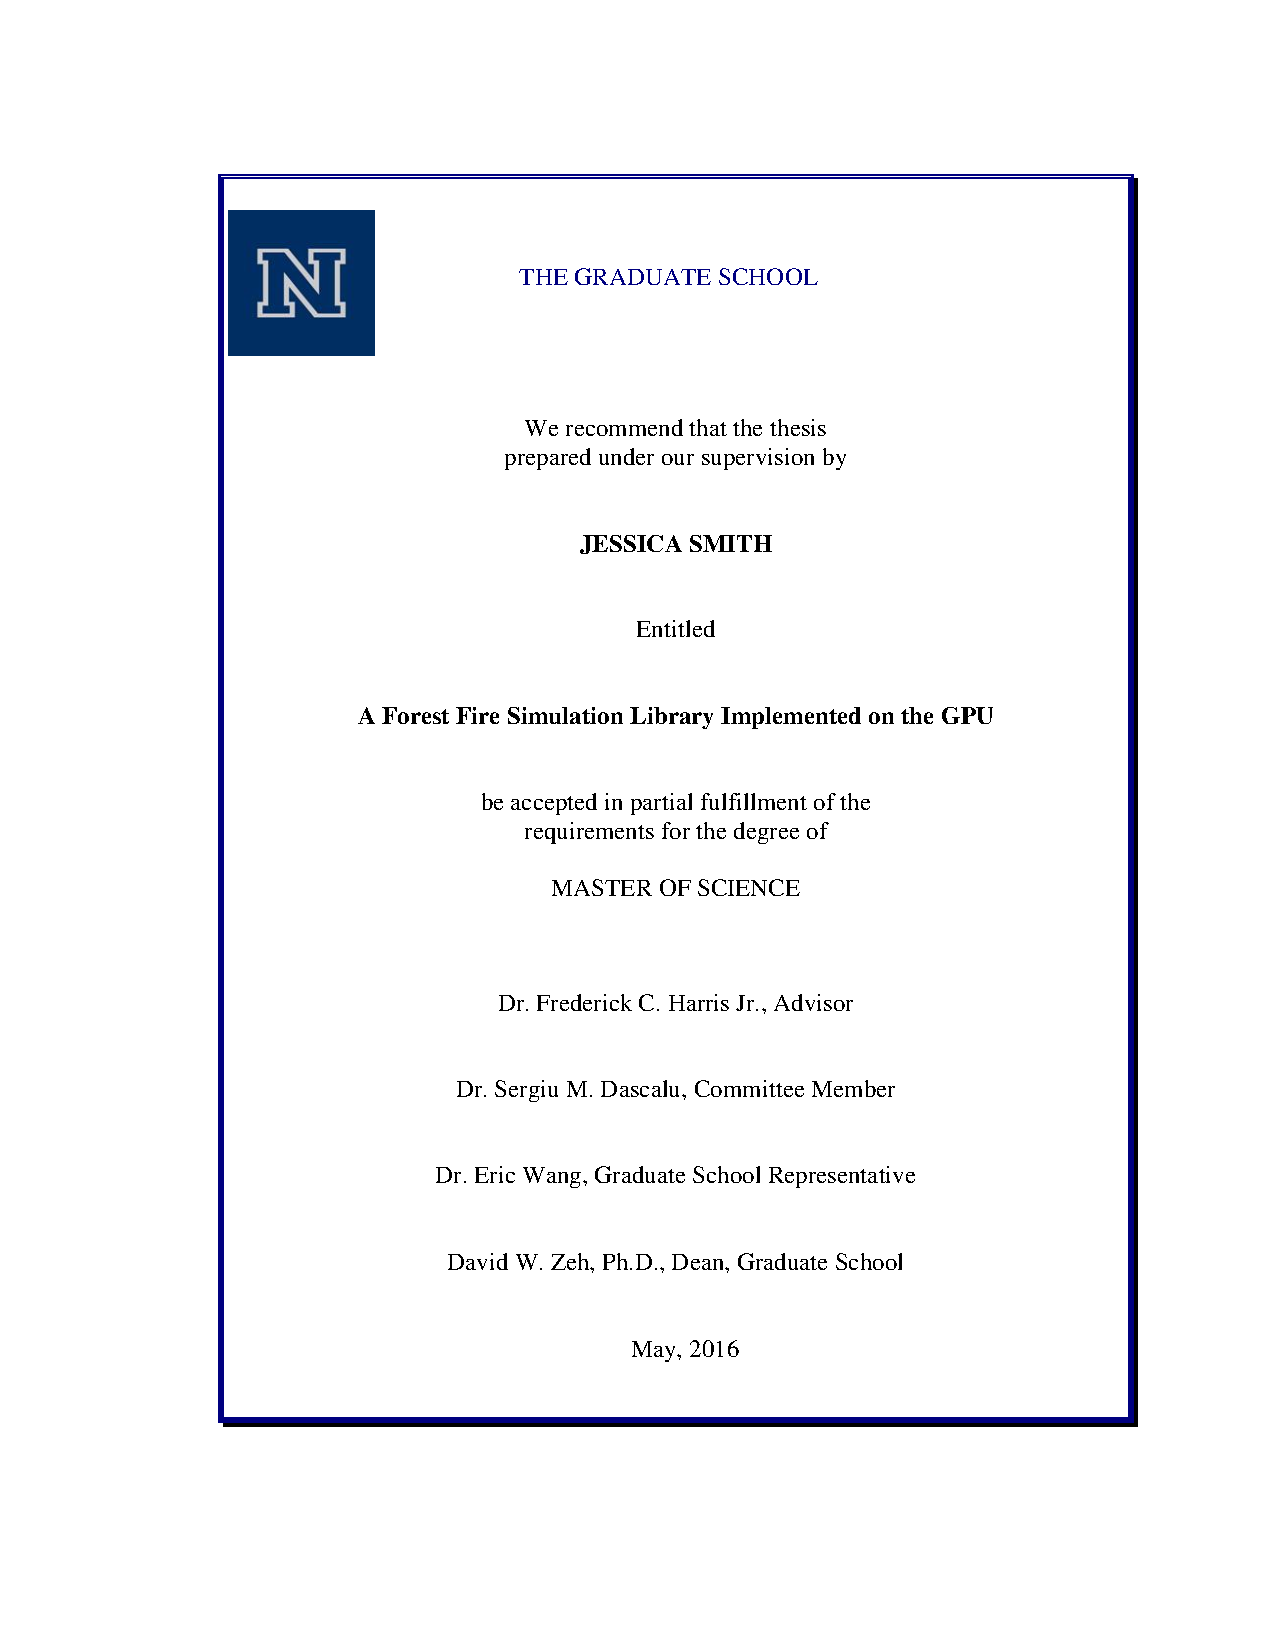
\includepdf[pages={1}]{figures/committee.pdf}
  \setcounter{page}{1}
  \pagenumbering{roman}
\newpage
\addcontentsline{toc}{chapter}{Abstract}
\begin{center}
  {\bf Abstract}
\end{center}

Forest fire simulation is a complex problem that requires an enormous amount of data processing. In order to operate a spread calculation in real-time, it becomes necessary to use parallel processing. Processing the spread calculations on the Graphics Processing Unit (GPU) allows hundreds of calculations to be performed at the same time, which allows the simulator to run up to 20X faster than its sequential counterpart. When the timings take up to half an hour, 20X faster makes the runtime feasable for a real-time application. This forest fire simulation library has the ability to incorporate base fire spread, fire acceleration, crowning, and a spotting prototype into the spread simulation. Three different methods for fire spread have been implemented to provide different perspectives to fire researchers. 
\newpage
\addcontentsline{toc}{chapter}{Dedication}
\begin{center}
\textbf{Dedication}

\vspace{0.2in}
To Madeline and Melody and Lily, my mini future coding army.
\end{center}

\newpage
\addcontentsline{toc}{chapter}{Acknowledgments}
\begin{center}
  \bf {Acknowledgments}
\end{center}

I would like to thank Dr. Fred Harris, Dr. Sergiu Dascalu, and Dr. Eric Wang for being on my committee, with special thanks to Dr. Fred Harris for giving me the opportunity to do research in the HPCVIS lab. I would like to thank Dr. Roger Hoang for providing the original groundwork for this research. I would also like to thank Chase Carthen for his assistance in debugging my project even though he was not directly assigned to it, and his assistance with GDAL. I would also like to thank Thomas Rushton for helping me brainstorm and keeping me sane. I would like to thank all my other labmates for listening patiently as I bounced ideas off them. 

This material is based in part upon work supported by: The National Science Foundation under grant number(s) IIA-1329469, and by Cubix Corporation through use of their PCIe slot expansion hardware solutions and HostEngine. Any opinions, findings, and conclusions or recommendations expressed in this material are those of the author(s) and do not necessarily reflect the views of the National Science Foundation or Cubix Corporation.

  % table of contents:
  % the .toc file generated isn't entirely accurate. If you run latex & bibtex a few times
  % so it generates everything, and look at the table of contents, it will show the list
  % of figures and list of rables page numbers to be on less than the actually are. To hack
  % a fix for it (assuming of course that it's really latex's fault and not mine), you can
  % open the .toc file and edit the numbers that will be displayed in the table of contents.
  % Then, run latex once. This will change the table of contents to the numbers you edited
  % in the .toc file. But running latex again will overwrite your changes.
  {
    \TOCSpacing

    \tableofcontents

    \newpage
    \phantomsection \label{totallyNotAHack1}
    \addcontentsline{toc}{chapter}{List of Tables}
    \listoftables

    \newpage
    \phantomsection \label{totallyNotAHack2}
    \addcontentsline{toc}{chapter}{List of Figures}
    \listoffigures

	% \nocite{*} % This line affects the bibliography.  If it is uncommented, then
				 % entries in the bibliography that aren't actually referenced in the
				 % paper will still be placed in the bibliography. Without this line,
				 % entries may still be placed in the .bib file, but the entries that
				 % are not used throughout the paper are no added to the created
				 % bibliography pages.
  }

  % actual text
  {
	\newpage
	\setcounter{page}{0}
	\pagenumbering{arabic}

	\BodySpacing

	\chapter{Introduction}

Every year, fighting forest fires costs taxpayers in the United States millions of dollars. From 2002 to 2012, the average amount spent per year on forest fire suppression by the federal government was \$962 million, which only amounted to 32\% of the entire federal wildfire protection funds \cite{forestcost}. This cost only covers the federal funds that are spent on fighting and preventing forest fires. It does not include the individual and environmental cost of loss of property and habitat. The highest cost that occurs during the efforts to fight a forest fire is the loss of life incurred by fire fighters. The ability to better predict the behavior of a wildfire greatly increases the effectiveness of fire fighting efforts, thereby reducing all the costs incurred during a forest fire. Another application domain for forest fires is the training of fire fighters. A sample forest fire could be provided in training scenarios which would allow fire fighters to have as close to hands-on forest fire training before they are exposed to real wildfires. 

In order to simulate wildfires, scientists have developed several methods for modeling the propagation of fire \cite{roth,BEHAVE,1983roth}. These fire models are based on the properties of the environment in which the forest fire takes place. Such properties include, but are not limited to, fuel load, fuel type, wind, live moisture, dead moisture, and crown height. Incorporating these and other variables into spread models can allow for accurate prediction of where a fire will spread and how quickly it will arrive. Research into developing fuel and moisture models is active to this day. These models provide the basis for the properties on which forest fire simulation is based.

The ability to realistically simulate forest fires is desirable because it allows fire experts to more accurately predict the impact of their fire-fighting decisions. Possible manipulations to the wildfire environment include adjusting moisture content to simulate a water drop, adjusting fuel loads where a simulated bulldozed treeline could exist, or reverse spread testing in which a fire started by firefighters would burn the fuel away from the advancing wildfire. Unfortunately, the amount of data required for realistic fire simulations requires a large amount of computation time to produce an accurate simulation. The more accurate and fine-grained the simulation, the longer it takes to process the data. A forest fire is a dynamic entity, therefore the ability of a simulator to run in real time is necessary for it to be an effective tool. The more complex and accurate a simulator is, the more useful it is to fire scientists. There are multiple aspects to accurately modeling the spread of a forest fire. The main four fire properties which influence the spread of a fire are base fires, crown fires, fire acceleration, and spotting \cite{firereview}. 

Using the GPU as a general purpose computing device has become popular in recent years, especially on problems which require a large amount of data processing. The GPU is ideally suited to high volume data processing applications because it can processes millions of inputs simultaneously, while a CPU may only process up to a few at a time \cite{cudabyexample}. This work has developed a fire simulation library which allows a user to run base propagation with fire acceleration tests on real-world data, as well as testing the crowning conditions and a simple spotting method. 

The remainder of this paper is structured as follows. Chapter \ref{chapter:background} contains the background information on forest fire models and the existing forest fire simulators. Chapter \ref{chapter:gpuSim} outlines of the work accomplished in this paper. Chapter \ref{chapter:design} presents the main components of the library's software specifications and design. Chapter \ref{chapter:implementation} describes the implementation details of the forest fire simulation library. Chapter \ref{chapter:results} presents the results of the timing tests and fire simulations performed for this work. Finally, Chapter \ref{chapter:conclusions} presents ideas for future enhancements for the fire library. 
    \chapter{Background and Related Work}
\label{chapter:background}
This chapter outlines the history of the work done in the research area of forest fire modeling and simulation. It then gives some background information on GPU computation as well as the fuel models used by this research.

\section{Fire Models}
\subsection{Overview}
The most widely used fire model is that developed by Richard C. Rothermel. His model of fire spread model depicts fire spreading in an elliptical shape. Rothermel also developed the first eleven fuel models that are still used to this day \cite{roth}. A fuel model is a model of a small region of forest and the vegetation it contains. Examples of vegetation types that are modeled by the fuel models are grass and grass-dominated regions, chaparral and shrub fields, timber litter, and stash \cite{1983roth}. The method by which the first eleven fuel models were created is the basis for the development of all modern fuel models. The fuel model contains information on properties of the forest in a particular region, and at a certain granularity. The forest is broken up into cells, each cell having properties which are modeled in the fuel model. For example, one fuel model might describe a coniferous forest in regions of 30x30 meter cells. These cells are what make up the basis for a fire simulation. 

\subsection{Taxonomy of Fire}
There are three types of fire models: theoretical, empirical, and semi-empirical \cite{firereview}\cite{firereview2}. Empirical models use statistical descriptions of wildfires and do not attempt to include any real-world observations into their models. These models are mostly concerned with the shape of a fire. However, their lack of incorporation with physical data mean they are not as useful outside of controlled environments. Semi-empirical models incorporate some of the statistical modeling found in emperical models but also include experimentally derived approximations to portions of the models. Rothermel's spread equations are an important example of the semi-empirical fire models \cite{roth}. More detail on Rothermel's equations will follow in subsequent sections. The final type of models are theoretical, which rely solely on physical principles. Their limitation occurs at the boundary of what data is available. This work implements semi-emperical methods for calculating fire spread.

\subsection{Fire Shape}
The majority of the existing forest fire simulators, including this work, calculate wildfire spread based on the Rothermel's fire spread equations \cite{roth}. More detail on the simulators which use this fire spread model will be covered later in the section. Equation \ref{eq:roth} shows his rate of spread equation, which is based on several parameters. 

% \begin{equation}\sum_{i=0}^{\infty}x_i=\int_{0}^{\pi+2} f\end{equation}
\begin{equation} \label{eq:roth}
R = \frac{(I_{p})_{o}(1 + \phi_{w} + \phi_{s})}{\rho_{b}\varepsilon Q_{ig}}
\end{equation}

Where R is the rate of spread, $(I_p)_o$ is the no-wind propagating flux, $\phi_w$ and $\phi_s$ are the additional propagating flux introduced by wind and slope respectively. The product of $\rho_b$ and $\varepsilon$ is referred to as the effective bulk density. The effective bulk density models the amount of fuel per unit volume of the fuel bed raised to ignition ahead of the advancing fire. $Q_ig$ is the heat of preignition (the heat required to bring a unit weight of fuel to ignition). These values are derived from or contained in the fuel model that describes the cell for which the computations are being done. 

The desired output from a forest fire simulator is a time of arrival map. Each cell in this time of arrival map represents a cell in the simulation forest, and the value it contains is the time at which the cell ignited and started propagating the fire. Once a cell is lit, it begins contributing to the spread of the fire to the surrounding cells and continues burning until the fuel in that cell is entirely used. The method of propagation may vary between simulators, but the basic spread rate is usually based on Rothermel's equations.

\subsection{Surface Fire}
There are several potential approaches to calculating the propagation of the fire. This propagation also determines the method for stepping through time in a simulation. This work implemented three methods for iterating through a simulation to calculate the time of arrival map. The first two spread methods (Minimal Time and Iterative Minimal Time) are based on stepping through time independent of specific fuel conditions and are based on the paper by Sousa, dos Reis, and Pereira \cite{gpufire}. The third spread method implemented in this paper (Burn Distances) was based on code and methods found in vFire \cite{vFire}. 

vFire implemented an accurate spread rate calculator based on Rothermel's fire spread equations and the fire spread and fuel model data to propagate based upon the physical burning of fuel. The Burn Distances propagation method was based on their work.

Sousa, dos Reis, and Pereira also used the GPU to improve their running times and ported fireLib to the GPU \cite{gpufire}, but were the first to use the parallel programming language CUDA \cite{cuda}. They implemented three kernels in which they explored three different propagation types. The propagation methods labeled Minimal Time and Iterative Minimal time are based on their work. 

\begin{figure}%[!t]
\centering
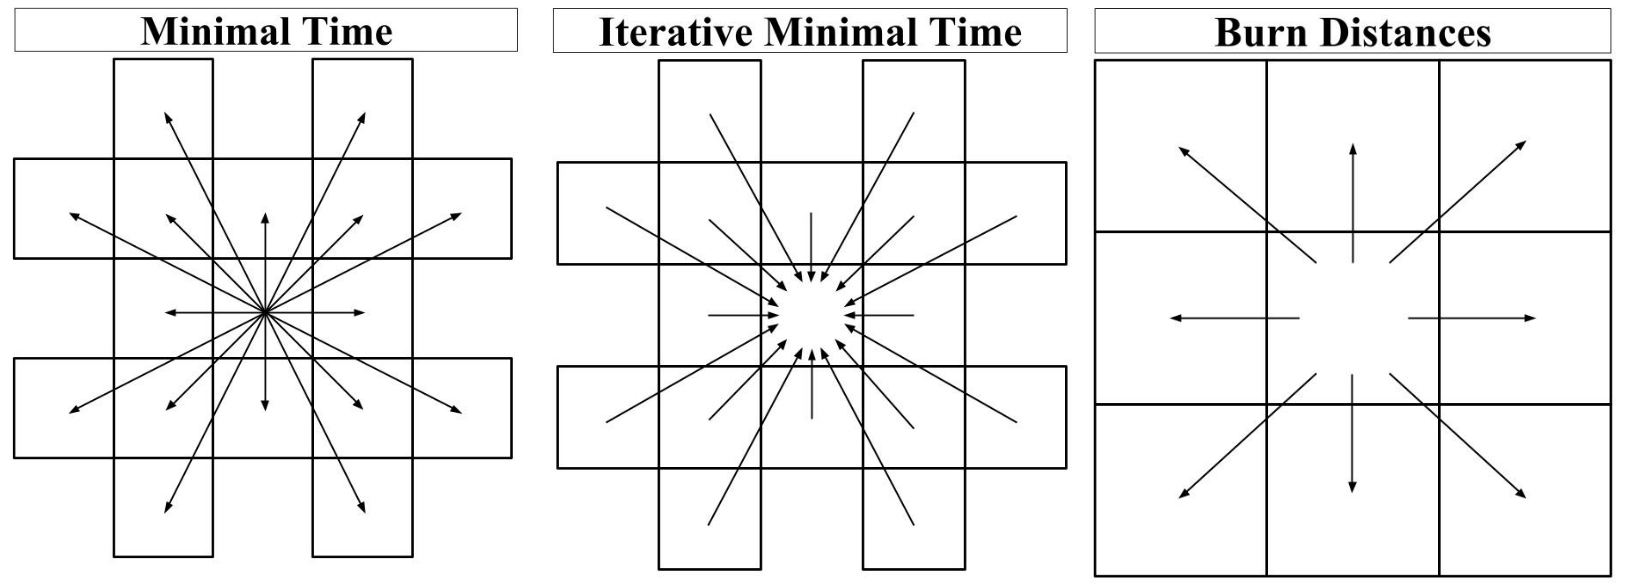
\includegraphics[width=\linewidth]{figures/background/spread_methods.PNG}
\caption{Neighbor access methodology for each of the propagation methods. From left to right: Minimal Time, Iterative Minimal Time, Burn Distances}
\label{fig:spreadTypes}
\end{figure}

\paragraph{Burn Distances}
The Burn Distances (BD) method is based on the idea that it takes a certain amount of time for fire to burn the distance between two cells. A distance is set as equivalent between all cells before the simulation burning may progress. The distance between cells is based on the properties of the forest model which is based on the size of the forest cell. The simulation iterates at a constant time step, and the amount the distance has burned is tracked throughout all the time steps. In this spread method, a cell looks to see which of its neighbors are on fire and which of those neighbors will burn the distance between the two cells first. The first cell to burn the total distance ignites the center cell as seen in Figure \ref{fig:spreadTypes}. In this work, the BD propagation method is based on work by Roger Hoang's vFire \cite{vFire}. The paper by Sousa, dos Reis, and Pereira also implemented a similar method, but it was not the basis for this propagation method in this work \cite{gpufire}.

\paragraph{Minimal Time}
The Minimal Time (MT) propagation method uses a dynamic time stepping method to step through the simulation. At each time step, a cell is examined to see if it is on fire. If the cell is burning, then the neighbors of the cell are examined as seen in Figure \ref{fig:spreadTypes}. If the neighbor is already on fire, it is ignored. If the neighbor is unlit, then the time of arrival for that cell is computed using the propagation equation found in Equation \ref{eq:rate}. In the Minimal Time method, time is incremented dynamically. Each time a new ignition happens, the ignition time is compared to the current 'timeNext' variable. If the new ignition time is smaller (the fire arrives sooner) than the current timeNext, then it replaces the timeNext value. This methodology means that time is incremented based on which cell will ignite the earliest. In the paper by Sousa, dos Reis, and Pereira, this method achieved the slowest speedup of their three methods \cite{gpufire}.

\paragraph{Iterative Minimal Time}
The Iterative Minimal Time (IMT) method is designed to avoid data dependencies. Each cell operates independent of its neighbors, calculating the ignition time based on the spread rates, and only finishing when the values between step $k$ and $k + 1$ converge. Each cell looks at the minimal time for each of its neighboring cells to burn towards it as shown in Figure \ref{fig:spreadTypes}. The value is known to converge after the difference between two time steps is less than some small threshold. The most appropriate value for this threshold can be determined through experimentation. In the work by Sousa, dos Reis, and Pereira, this method achieved the highest speedup of their three methods \cite{gpufire}. 

\subsection{Crowning}
Crowning is the phenomena of the fire moving from spreading along the base of the forest to up the trees to their crowns. There are two types of crowning: passive and active. A passive crown fire is one which does not spread to the overall propagation of the fire. Conversely, an active crown fire does contribute to the spread of the fire. The modeling method used for this implementation will be discussed in the Implementation section of this paper. The method for calculating crowning in this library was based on the work found in vFire \cite{vFire}. vFire based their implementation on the work found in FARSITE \cite{FARSITE}, which implemented their methods based on the work done by Van Wagner \cite{wagner1977}\cite{wagner1993}.

\subsection{Spotting}
Spotting occurs when fire brands from the wildfire are lifted into the air and fly ahead of the advancing flame wall to start new fires. This incident occurs when Torching occurs. Torching occurs when the fire spreads from the base of the forest to the tree-tops. It does not contribute to the spread of the fire. This method was implemented based on the work found in FARSITE \cite{FARSITE}. FARSITE based their implementation on the model developed by Albini in 1979 \cite{ablini}. The implementation found in this work had to be simplified somewhat because of constraints on the data available to the researchers. Details on the limitations found in spotting may be found in the Implmentation chapter of this paper. 

Another paper which implemented spotting did not use the same empirically-based methodology as the method used by FARSITE and in this paper. The work by Koo, Linn, Pagni, and Edminster implements a method for spotting based on the theoretical models known about physical phenomena surrounding wildfires \cite{firetecSpotting}. They experiment with different sized and shaped fire brands to determine the impact they have on the spotting distance possible during a forest fire. 

\section{Fire Simulators}
Since Rothermel's paper was published in 1972, several fire spread simulators have been developed. Nearly every major forest fire simulator has used his spread equations as the basis for their simulation. 

\subsection{BEHAVE}
The first major fire spread simulator was developed in 1986 called BEHAVE\cite{BEHAVE}. BEHAVE used Rothermel's fire propagation methods \cite{roth}. BEHAVE had two main functions to the application. The first function allowed users to load in fuel models from Rothermel's paper, but also to develop and save new fuel models. The simulator then had the ability to integrate the newly developed fuel models in its simulations. The second function of the application would run a simulation and burn prediction on the desired fuel model. The usefulness of the BEHAVE simulator is that it gives a realistic viewpoint of how a fire would behave given a specific fuel model at a specific instance in time. The output of this simulator appeared in a table which represented the times of arrival for each cell in the simulation. There was no visualization method available for this simulator. The simulation was meant to be used as a training tool rather than a real-time tool to be used to fight wildfires. It is still used to this day by fire scientists who are not familiar with the programming requirements of the newer simulators that have been developed. It remains a useful tool for fuel model development. 

\subsection{fireLib}
A decade later in 1996, BEHAVE was the basis for a new forest fire library that was developed using the programming language C called fireLib \cite{fireLib}. The code was based entirely on BEHAVE's simulator, but brought up to a then-modern platform. FireLib can run much faster than BEHAVE, and the output is given in time of arrival arrays rather than a table. Each [x,y] in the array corresponds to a cell in the fire simulation, and the time of arrival is the time at which the cell ignites, and can then begin to propagate the fire. The fire library is more flexible than BEHAVE and allows a user to design their own methods for propagating the fire. There are a few different methods which may be used, and will be addressed later in the paper. However, where BEHAVE was an entire application which had an interface component, fireLib is simply an open source forest fire library and both the visualization and interface development are left up to the user. fireLib incorporates the element of time that BEHAVE is missing, allowing researchers to look at a fluid time scale rather than a single instance of a fire. 

\subsection{FARSITE}
In 2004, FARSITE was developed, which works as a full-scale forest fire simulator \cite{FARSITE}. It has been continuously developed since 2004 and is currently still operational. It incorporates more features than simple fire spread, such as crown fires, surface fires, fire acceleration, and spotting. While it is one of the most advanced and accurate forest fire simulators, it is not very fast. The FARSITE simulator runs entirely sequentially, which it will be shown how slow a sequential implementation of these methods are later in this paper. Despite the lengthly amount of time required to compute its simulations, it is one of the most widely used forest fire simulators in existence today. A benefit of using FARSITE over other options is that they are able to incorporate advanced geospatial data.

\subsection{vFire}
This paper used much of the fire spread implemenation from a forest fire simulator called vFire \cite{vFire}. vFire was based on hFire, and are both cellular based spread models. They run faster than FARSITE, but do not have the same level of precision \cite{hFire}. vFire was the first forest fire simulator to utilize the parallel nature of the GPU to run calculations on the fire spread. At the time of its development, the only way to program on the GPU was to use the programming language OpenGL \cite{opengl}. vFire used the shader language glsl to utilize the multicore abilities of the GPU. vFire implemented a technique that has dynamic time stepping to burn distances between cells to determine an accurate time of arrival for the fire spread. The important feature that vFire accomplished was po\begin{figure}%[!t]
\centering
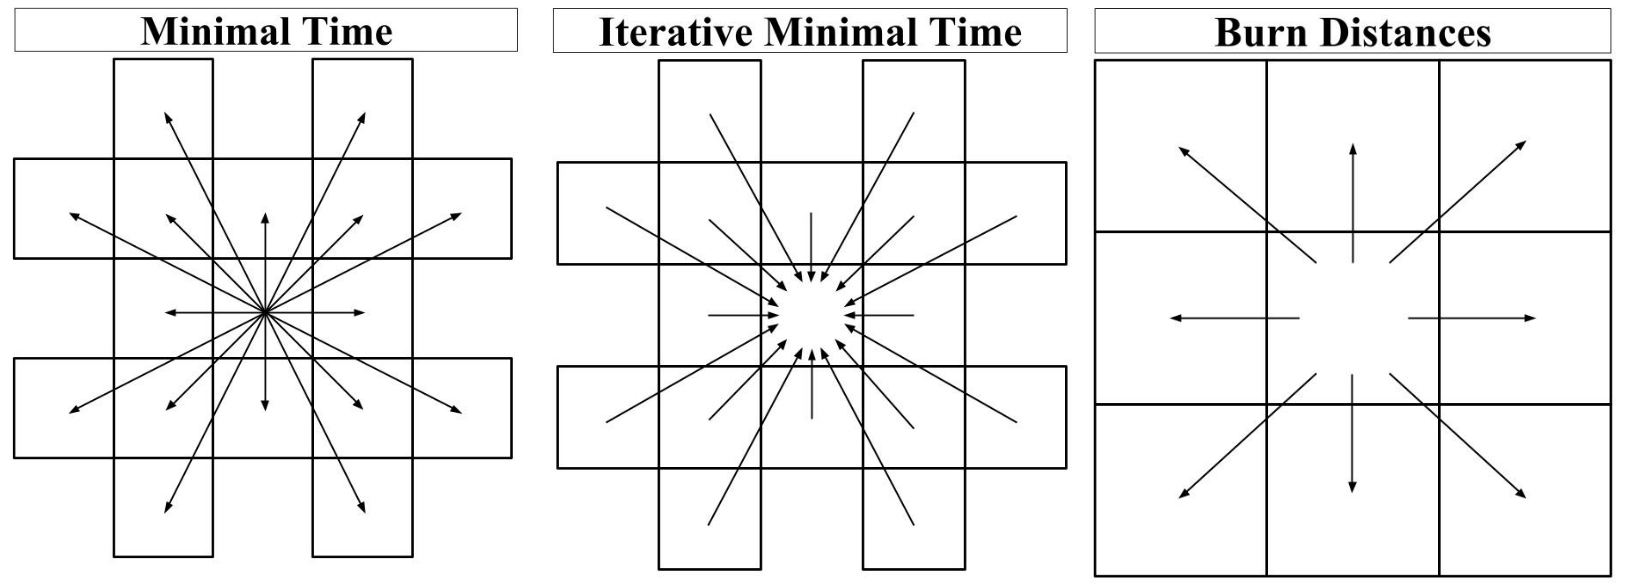
\includegraphics[width=\linewidth]{figures/background/spread_methods.PNG}
\caption{Neighbor access methodology for each of the propagation methods. From left to right: Minimal Time, Iterative Minimal Time, Burn Distances}
\label{fig:spreadTypes}
\end{figure}rting the computation of the fire spread to the GPU using OpenGL shaders \cite{opengl}. This simulator did not implement a sequential version to compare results against, and so there is no data to support how much improvement in runtime it accomplished. 

\subsection{FIRETEC}
Researchers at Los Alamos National Laboratory have created a fire simulator which is not based on the elliptical spread equations developed by Rothermel. Rather than using semi-empirical data to calculate their spread methods, they use theoretical models of chemical reactions and heat transfers to descipher where the fire is going to propagate \cite{firetech}. This method for calculating spread is very computationally expensive, and is used mainly for research purposes at the moment. 

\section{GPU Computation}
\subsection{Overview}
% History from CUDA site:
% http://www.nvidia.com/object/cuda_home_new.html
GPU's were originally designed as graphics accelerators supporting only very specific fixed-function pipelines. This meant that using them for high performance computation was not easy unless it could be integrated with some sort of visualization language. An example of such an integration may be seen in vFire \cite{vFire}. In 2006, NVIDIA released CUDA, which was the world's first solution to general-purpose computing on the GPU. Ever since its release, and even beforehand, the GPU was used for its high-processing capabilities. The architecture of the GPU allows for hundreds of low-powered processors to run in parallel. This type of computation is ideal for situations where the same computation to hundreds of inputs. The pitfalls of GPU computation occur when data dependencies exist in the data. If one portion of the data must wait on another to finish, it limits the usefulness of the GPU for processing. 

\subsection{CUDA}
CUDA is a parallel computing platform and computing model created by NVIDIA \cite{cuda}. It harnesses the hundreds of cores provided by a GPU an allows programmable kernels to be written. A kernel is a small bit of code that is run by a thread on the GPU. In the world of GPU programming, there is host data and device data. Host data is data which is stored on the home machine and processed by the CPU. Device data is data which is copied to the GPU for processing \cite{cudabyexample}. The architecture of a GPU that can be accessed through CUDA begins at the grid level. A single thread is assigned a thread ID. Each thread ID is unique among its block, which contains a certain number of threads. Many current GPUs have blocks that can contain up to 1024 threads. There may be many blocks in a single grid of a GPU, and the blocks may be assigned. The total number of threads would then be the number of blocks multiplied by the number of threads per block \cite{cuda}. An outline of the heterogeneous programming style may be seen in Figure \ref{fig:cuda_arch}. 

\begin{figure}%[!t]
\centering
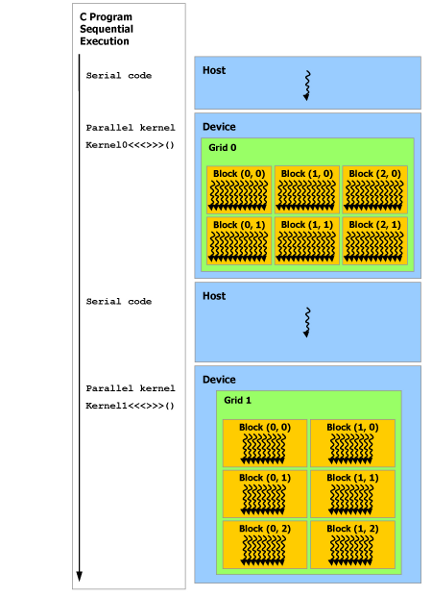
\includegraphics[height=7.5in]{figures/background/cuda_arch.png}
\caption{Outline of the programming style between the CPU and GPU \cite{cuda}.}
\label{fig:cuda_arch}
\end{figure}

In order to test the work presented in this paper, the tests were run on a CUBIX box \cite{cubix}. The CUBIX box is designed to leverage multi-GPU and CPU programming. The box contains seven GPUs and four CPUs. This work only implements single-GPU simulations. The reason the CUBIX box was used was for the speed of determining results. It allows several simulations to be run and timed simultaneously, which meant the results could be gathered faster. 

\section{Fuel Models}
The data needed to process the fire simulation begins with the Fuel Models required by the simulator. Rothermel developed thirteen original fuel models, which are still used today \cite{1983roth}. Additional fuel models have been developed since that time, 42 of which are incorporated into this work. Additional fuel models, including those of what are called 'unburnable' in this work may be found in the work by Scott and Burgan \cite{fuelmodels}.  The fuel models contain data regarding surface-area-to-volume ratio by class and component, fuel model type, fuelbed depth, extinction moisture content, and fuel particle heat content. These data types are used to determine the behavior of the fire in a particular cell of the simulation. The details on the data available may be found in the documentation of the library. 
    \chapter{Real-time GPU-based Wildfire Simulation}
\label{chapter:gpuSim}
I NEED A CATCHY NAME FOR MY SIMULATOR. 

XXX is a wildfire simulation library that allows the user to take advantage of the highly-parallel nature of the GPU. The propagation, crowning, and spotting are all implemented both sequentially and as kernels on the GPU using the programming language CUDA \cite{cuda}. 

The GPU is ideally suited to this type of computation because every cell that is propagating must process the same computations as its propagating neighbors. 


    \chapter{Analysis and Conception}
\label{chapter:design}

\section{Overview}
The vFireLib library provides functions that allow for a dynamic forest fire simulation to occur. The library is responsible for managing the data provided by input files by a user, calculating spread data, running the sequential or parallel simulation, and writing out the final data to a file for further reading. The diagrams in this section of the paper were generated using the Creately web interface for generating UML diagrams \cite{creately}. 

\section{Service Requirements}

\subsection{Functional Requirements}
The functional requirements were created from the behavioral requirements of the library's functionality as used by an outside source. The list of functional requirements may be viewed in Table \ref{tbl:functional_reqs}. The software engineering steps used in this work were based on the work accomplished by Ian Sommerville in his Software Engineering book \cite{softwareengineering}.

\begin{table}
\caption{vFireLib Wildfire Simulation Library Functional Requirements.}
\label{tbl:functional_reqs}
  \rowcolors{2}{gray!25}{white}
  \begin{tabular}{cl}
    \rowcolor{gray!50}
    Number & Description \\
    FR01 &  \begin{tabular}[c]{@{}l@{}}The library shall read in fuel model, moisture model, and\\ terrain data.\end{tabular}\\
    FR02 & The library shall define the granularity of simulation size. \\
    FR03 &  \begin{tabular}[c]{@{}l@{}}The library shall create and initialize all data members necessary\\ to a complex simulation on the CPU and GPU.\end{tabular}\\
    FR04 & The simulation shall calculate the maximum rate of spread for every cell. \\
	FR05 & \begin{tabular}[c]{@{}l@{}}The library shall run a GPU simulation using the BD, MT,\\ or IMT spread methodologies. \end{tabular}\\
    FR06 & The library shall calculate fire acceleration for the simulation. \\
    FR07 & The library shall allow the Crowning flag to be toggled. \\
    FR08 & The library shall allow the Spotting flag to be toggled. \\
    FR09 & \begin{tabular}[c]{@{}l@{}}The library notify the user when their input files are not compatible\\ with the simulation system. \end{tabular}\\
    FR010 & The data must be initialized before the simulation is run. 
  \end{tabular}
 % \end{table}
%\begin{table}
\\ \\
\caption{vFireLib Wildfire Simulation Library Non-functional Requirements.}
\label{tbl:nonfunctional_reqs}
  \rowcolors{2}{gray!25}{white}
  \begin{tabular}{cl}
    \rowcolor{gray!50}
    Number & Description \\
    NR01 & The library shall be written in C++ and CUDA. \\
    NR02 & The library must use CUDA version 6.0 or higher. \\
    NR03 & \begin{tabular}[c]{@{}l@{}}The library's sequential implementation must be a direct reflection of its\\ parallel implementation. \end{tabular}\\
    NR04 & \begin{tabular}[c]{@{}l@{}}To run the parallel version of the code, an NVIDIA GPU with CUDA Compute\\ Capability 2.0 or higher is needed. \end{tabular}\\
    NR05 & This library must be used on the Linux platform. \\
    NR06 & The library must use GDAL version 1.10.1. \\
    NR07 & The library must be compiled with CMake Version 2.8 or higher. \\
  \end{tabular}
  \end{table}

\subsection{Non-functional Requirements}
The non-functional requirements were created based on the internal interactions of the library functions. Data needed to be manipulated and passed among classes and between the host and device for computation purposes. The non-functional requirements are listed in Table \ref{tbl:nonfunctional_reqs}.
  
\section{Use Case Modeling}
\subsection{Overview}
For a better understanding of how the user interacts with the library, this section describes use cases for running a simulation. These diagrams have been generated using the Unified Modeling Language \cite{UML}. Both the parallel and sequential functionalities will be shown here. The use case model may be found in Figure \ref{fig:usecase_diagram}. In order to better illustrate the library's functionality, a sequence diagram may be seen in Figure \ref{fig:sequence_diagram}. 

\begin{figure}
    \centering
    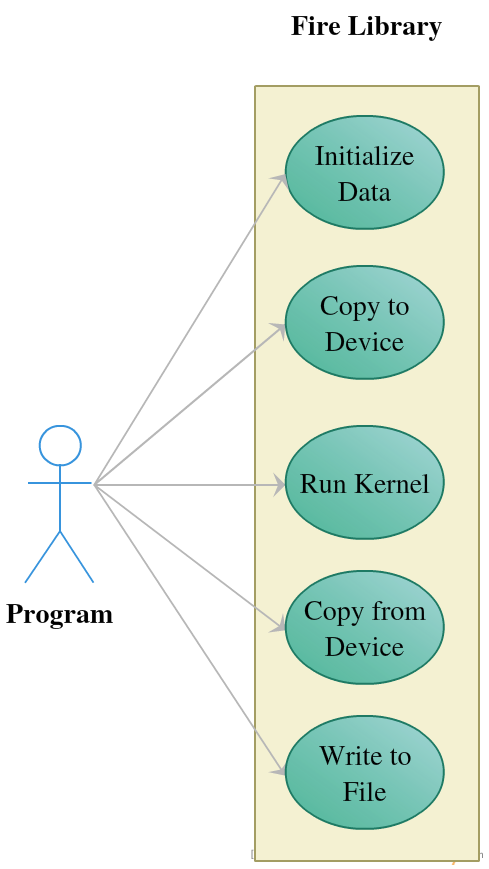
\includegraphics[height=4.5in,width=\textwidth,keepaspectratio]{figures/design/use_case_diagram.png}
    \caption{A use case diagram for the Wildfire simulation library.}
    \label{fig:usecase_diagram}
\end{figure}

\begin{figure}
    \centering
    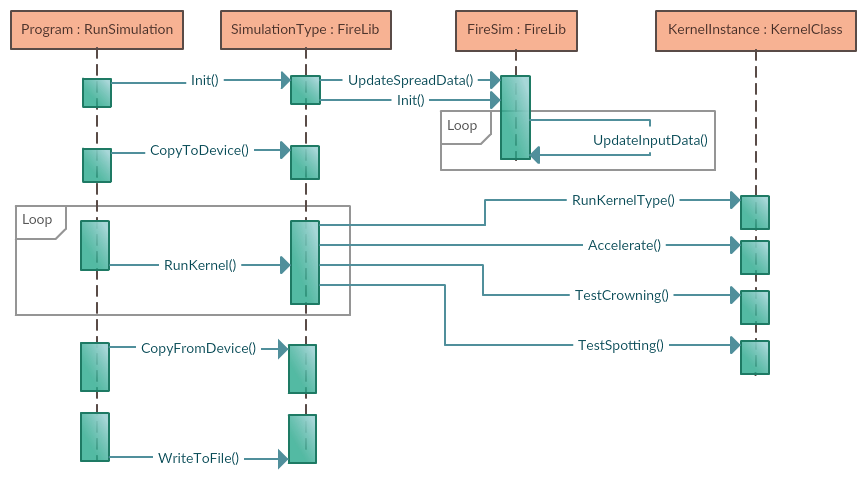
\includegraphics[height=\textheight,width=\textwidth,keepaspectratio]{figures/design/sequence_diagram.png}
    \caption{A sequence diagram for the Wildfire simulation library.}
    \label{fig:sequence_diagram}
\end{figure}

\subsection{Detailed Use Cases}
\subsubsection{Initialize Simulation Data}
The terrain data encompasses more than the terrain data. The fuel model data must be read from the files, the terrain data, the moisture data, the canopy height data, the crown base height data, and the crown bulk density data. If there is an error with any of these files, the library reports an error. This is the point where the simulation is scaled to the appropriate granularity. 

\subsubsection{Initialize CPU Data}
The data must be initialized from the input data into a format which is useable by the simulation. This includes calculating the maximum spread rate before the simulation begins. This function must be called whenever there is a change to the data values in the initialize function. 

\subsubsection{Copy To Device}
The data needed for the simulation must be copied from the host to the device (GPU). This must occur every time the data is changed on the CPU side of the library. 

\subsubsection{Propagate}
This occurs when a propagate function is called. This could be from three sources: BD, MT, or IMT. 

\subsubsection{Accelerate}
Once the fire has spread after a time tick, the rate of spread from the fire is accelerated.

\subsubsection{Crowning}
Once the fire has been accelerated, a test is done to see if the fire is crowning. The moment a fire crowns, the torching flag is set for one time tick. The crowning test also checks to see if the fire is passive. If it has progressed to an active fire, the maximum rate of spread is updated to reflect the change. 

\subsubsection{Spotting}
In the event that torching has occurred during the crowning phase, spotting is calculated. A fire brand is launched into the air and it is tested to calculate if any new fires start ahead of the flame wall.

\subsubsection{Copy From Device}
On completion of the desired simulation, the data from the simulation must be copied back from the device back to the host for further processing. 

\subsubsection{Write To File}
This functionality allows the user to write the computed output of their time of arrival map to a .csv output file. 

\section{Architecture}
This library is designed to act as a facilitation tool that will allow a user to program their own custom-defined simulations. The program aims to make visualization easily portable to users. In order to convey an understanding of the overall architecture of the library, a class diagram is provided to describe the system in Figures \ref{fig:class_diagram} and \ref{fig:fire_sim_class_diagram}:

\begin{figure}
    \centering
    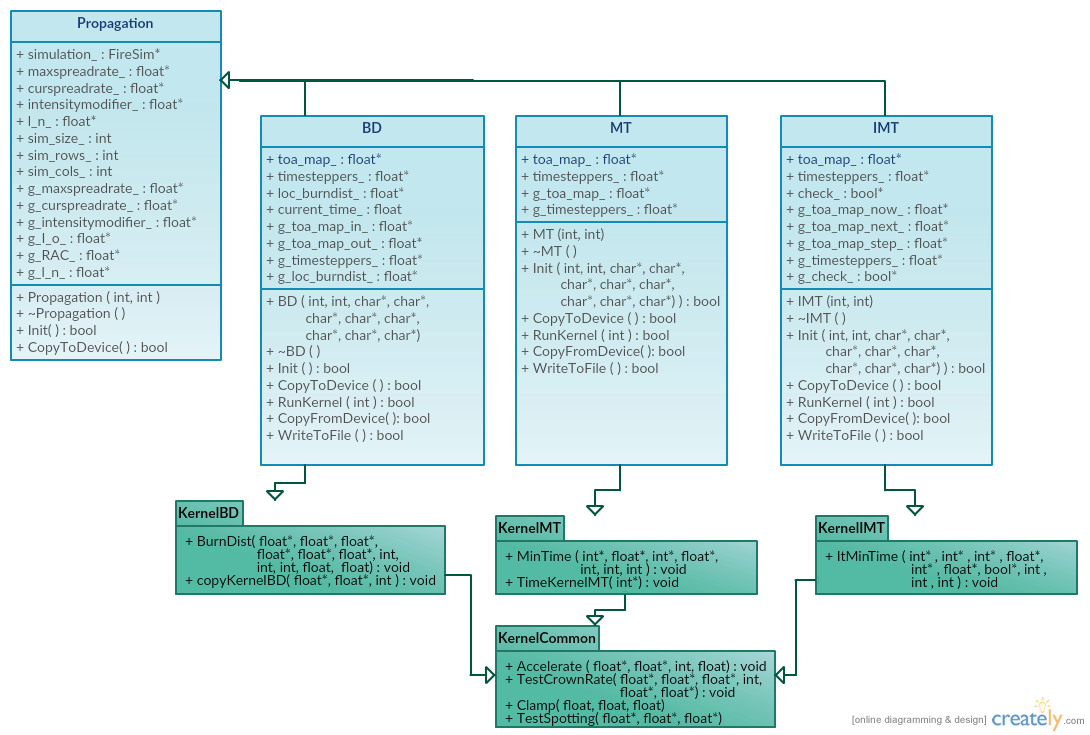
\includegraphics[width=\textwidth,keepaspectratio]{figures/design/class_diagram.png}
    \caption{A class diagram for the Propagation classes in the simulation library.}
    \label{fig:class_diagram}
\end{figure}

\begin{figure}
    \centering
    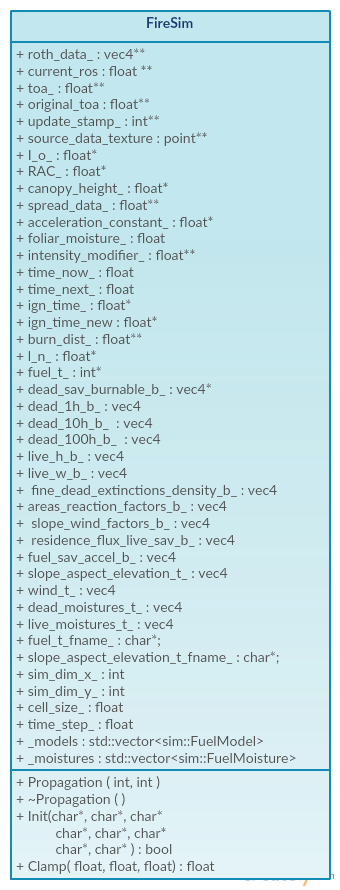
\includegraphics[height=\textheight,keepaspectratio]{figures/design/fire_sim_diagram.png}
    \caption{A class diagram for the Propagation classes in the simulation library.}
    \label{fig:fire_sim_class_diagram}
\end{figure}

    \chapter{Implementation}
\label{chapter:implementation}

\section{Overview}
Once the preprocessing is complete, one of three simulation methods was applied: Minimal Time, Iterative Minimal Time or Burn Distances. Since the goal of a forest fire simulator is to operate in real-time, it is unrealistic to expect to wait that long to receive the simulation data. After thirty minutes, the fire will have changed enough for the simulation's predictions to be irrelevant. The following algorithm outlines the simulation steps from start to finish:

\begin{algorithm}
  \caption{Simulation Progression}
  \label{alg:sim}
%   \begin{algorithmic}[1] <- this will give you line numb
  \begin{algorithmic}
  \STATE InitializeTerrainData();
  \STATE CalculateSpreadRates();
  \WHILE{Simulation !Complete}
  \STATE RunPropagationSimulation();
  \ENDWHILE  
  \STATE GenerateOutputFile();
  \end{algorithmic}
\end{algorithm}

The InitializeTerrainData() and CalculateSpreadRates() functions in Algorithm \ref{alg:sim} are part of the preprocessing in this project. These are not addressed in detail in this paper due to space constraints. The RunPropagationSimulation() portion is the focus of this paper and will be outlined in more detail in the following sections.

In order to address the runtime analysis needed for this paper, a sequential version of the kernels was also implemented. The equations and spread methodologies are the same between the kernels and the sequential implementation. However, many of the data concurrency problems were not a problem in the sequential version, and therefore some of the secondary kernels which will be addressed were not implemented in the sequential versions. The sequential implementations are not discussed in detail in this paper because they are not the main focus of the library and exist mostly for comparison purposes.  


\section{Surface Fire}
There are several potential approaches to calculating the propagation of a wildfire. This paper implemented three methods for iterating through a simulation to calculate the time of arrival map for a simple one-source forest fire under constant terrain and wind conditions. The first two spread methods (Minimal Time and Iterative Minimal Time) are based on stepping through time independent of specific fuel conditions and are based on the paper by Sousa, dos Reis, and Pereira \cite{gpufire}. The third spread method implemented in this paper (Burn Distances) was based on code and methods found in vFire \cite{vFire}. vFire implemented an accurate spread rate calculator based on Rothermel's fire spread equations and the fire spread and fuel model data to propagate based upon the physical burning of fuel.

The model for propagation rate used in this paper was the same for all three spread methods. The model is based on Rothermel's fire spread equations, and is found increately Equation \ref{eq:rate}. This equation was derived by the creators of vFire \cite{vFire}, and the data processing done in the preprocessing phase of this project was based on their work. The preprocessing step translates the equation from Rothermel's work seen in Equation \ref{eq:roth} to what is seen in the following Equation \ref{eq:rate}. The preprocessing data is out of the scope of this paper and is not covered in detail. 

\begin{equation}
r(\Theta ) = R_{max}\frac{1.0 - \varepsilon }{1.0 - \varepsilon cos(\phi-\Theta )}
\label{eq:rate}
\end{equation}

$R_{max}$ is the maximum rate at which a fire can spread. The scale at which it spreads is dependent on the input files. It will be in distance / time step size. In this implementation, this rate will be in meters/100 seconds. $\varepsilon$ is the eccentricity of the fire, which is based on wind and slope data. $\phi$ is the orientation. $\Theta$ is the direction in which the fire is spreading. $R_{max}$, $\varepsilon$, and $\phi$ are all computed based on the terrain data before the propagation simulation takes place. This is done in the preprocessing stage because the rates at each cell do not change until the forest model changes. An interactive simulator could potentially allow for these variables to change (i.e. modeling a water dump from a helicopter or a bulldozer tearing down a line of trees) but that is outside the scope of this research paper. To implement these features, changes would be made to the fuel and moisture models used to determine the possible rate of change in a cell. The direction $\Theta$ is computed based on which neighbor is being examined at the time. 

During the preprocessing phase, there are several data files which need to be processed and interpolated to be of the same size. The fuel data and slope data are stored in files containing interpolation data such as size of cell, width, and height of the data grid. The Geospatial Data Abstraction Library (GDAL) was used to interpolate the data from the terrain and fuel files into the desired size of simulation \cite{GDAL}. Wind data is incorporated into the spread rate calculations as a 2D vector for each cell in the grid. The wind data contains a direction and magnitude. The fuel models provide the detailed parameters by which the rate of of spread is calculated. There are potential areas in this processing phase (such as calculating the Rothermel spread properties) that could be parallelized to improve overall running times of this simulator. However, the focus of this paper was to explore the potential for calculating fire spread on the GPU, so these possibilities were not addressed and are left for future work. 


\section{Fire Propagation}
\subsection{Overview}
In a wildfire spread simulation, there has to be a way to iterate through time and check for the propagation of the fire. This thesis implemented three such spread methods, which provide different fireline shapes as they move through the simulation. Each of the propagation methods are written as CUDA kernels \cite{cuda}. The implementation details of each unique method follow in this section of the paper. The following figure, Figure \label{fig:spreadTypes_2}, is a repeat of Figure 2.1 for ease of reference to the reader. It depicts the neighbor access methods for the propagation methods.

\begin{figure}%[!t]
\centering
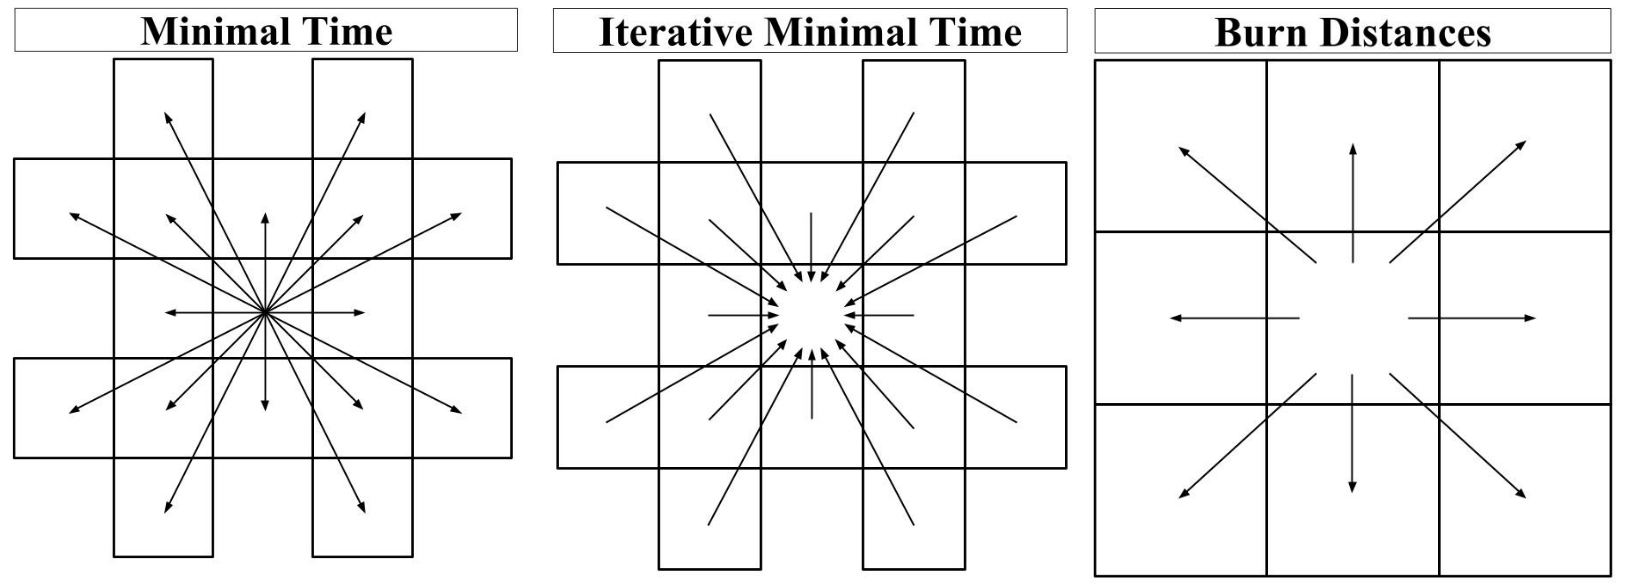
\includegraphics[width=\linewidth]{figures/background/spread_methods.PNG}
\caption{Neighbor access methodology for each of the propagation methods. From left to right: Minimal Time, Iterative Minimal Time, Burn Distances}
\label{fig:spreadTypes_2}
\end{figure}

\subsection{Burn Distances}
Burn distances is a kernel which simulates the burning of the physical distance between fire cells. In order to limit unnecessary computations, cells that are already on fire are skipped in the kernel. Only those that are not on fire check their neighbors to see if during this time step they are set alight.The pseudocode for the algorithm for the BD propagation method is found in Algorithm \ref{alg:BD}.

\begin{algorithm}[H]
  \caption{Burn Distances Algorithm}
  \label{alg:BD}
  \begin{algorithmic}
  \FOR{$cell = 0$ to $numCells$}
  \STATE $//$ Check to see not on fire
  \IF{$ignTime[cell] == INF$}
  \STATE $Skip$
  \ENDIF
  \STATE $//$ Check Neighbors for spread
  \FOR{$n = 0$ to $7$}
  \IF{$ignTime[neighborCell] < INF$}
  \STATE $Skip$
  \ENDIF
  \STATE $ROS$ = Compute ROS according to Equation \ref{eq:rate}
  \STATE $burnDistance$(totDist[neighborCell], ROS, timeStep)
  \IF{distance is burnt}
  \STATE $ignTime[neighborCell] = timeNow$
  \ENDIF
  \ENDFOR
  \ENDFOR
  \end{algorithmic}
\end{algorithm}

During each kernel call, each cell is processed independent of its neighbors. However, when a new cell ignites, the data must be written out to the vector somehow. There is no way to ensure which threads are reading and writing all at the same time. In fact, it was found that race conditions existed when the threads were reading from and writing to the same vector. In order to fix this problem, an input and output vector were created. Threads read only from the input vector and write to the output vector. A secondary kernel was written to copy the data values from one vector to another between the propagation kernel calls. The algorithm for the copy kernel may be found in Algorithm \ref{alg:BD_copy}:

\begin{algorithm}[H]
  \caption{Burn Distances Algorithm}
  \label{alg:BD_copy}
  \begin{algorithmic}
  \FOR{$cell = 0$ to $numCells$}
  \STATE $//$ Copy from output back to input 
  \STATE $InputVector[cell]$ = $OutputVector[cell]$
  \ENDFOR
  \end{algorithmic}
\end{algorithm}

An issue with this method arose from the static time step and needed to be addressed. Figure \ref{fig:accerr} shows the problem that can arise from the fixed time step. Figure \ref{fig:accerr} (a) shows the initial propagation. In this scenario, imagine that the propagation rate for b is much higher than a, but because the time step is large enough, they both propagate approximately one cell per time step. Figure \ref{fig:accerr} shows the second propagation step in time. In this example, a' propagates to a''. Because of the faster propagation rate of b, b' should propagate to b'' and b'' to b''' before a' propagates to a''. In the case where the time step is too large, the time of arrival would show an erroneous value for the cell holding a''. To fix this issue, the time step in the simulation must be set to a small enough value to avoid this error. The time step should be set to the smallest possible time it takes fire to propagate from one cell to another. 

\begin{figure*}
% \begin{figure}
\centering
%   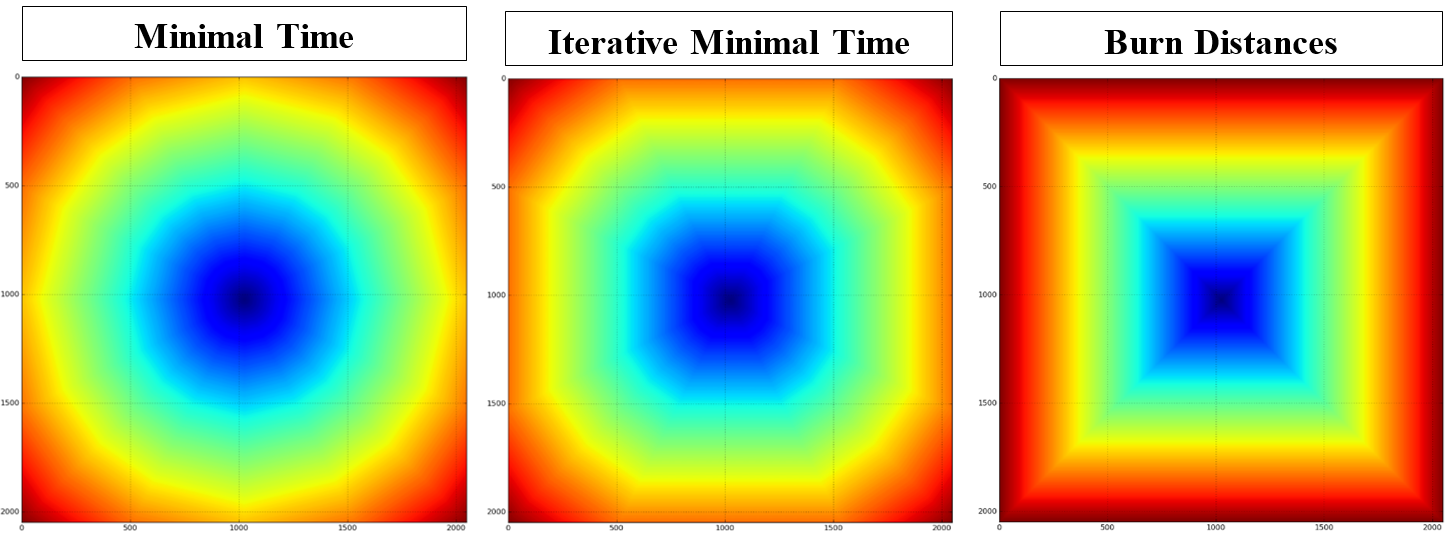
\includegraphics[width=\textwidth,height=4.2cm]{burn_patterns}
  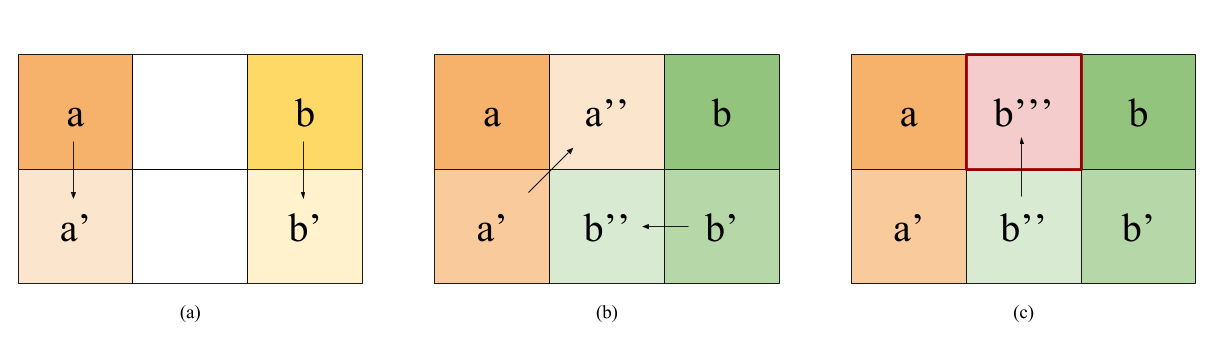
\includegraphics[width=\linewidth]{figures/implementation/Acceleration_error.png}
  \caption{The possible error for a fixed time-step propagation method. (a) shows the initial step with two lit cells a and b propagating to cells a' and b'. (b) shows a' propagating to a'' in the next time step. (c) is the situation where b'' would have propagated faster to the slot occupied in the previous step by a'', but because of the fixed time step, it would not propagate to an already lit cell.}
  \label{fig:accerr}
% \end{figure}
\end{figure*}

A cell ignites when the distance from an ignited neighbor has been completely burned. Each cell stores the distance that has been consumed by the fire in each direction to its neighbors. The simulation checks a cell's neighbors for ignition, and then uses their properties to burn the amount of distance in that time step towards the current cell as seen in Figure \ref{fig:spreadTypes_2}. The cell ignites when one of its neighbors burns the distance completely. The cell then inherits the properties of the fire that propagated to it. The equation to determine how much distance is burned can be found in Equation \ref{eq:burn}. 

\begin{equation}
d = d - r \Delta t
\label{eq:burn}
\end{equation}

Where $d$ is the distance that needs to be consumed. It is slowly decremented over time by the rate of spread ($r$) times the time step size ($\Delta$ $t$). In order to account for the fact that an 'overburn' could occur with fixed time steps. The exact time of arrival that is calculated is dependent on the exact time of arrival that the fire would have arrived at the cell. The equation used to find the exact time of arrival is found in Equation \ref{eq:overburn}. 

\begin{equation}
TOA = t_{now} + \frac{d_{over}}{r}
\label{eq:overburn}
\end{equation}

Where $TOA$ is the time of arrival that is written out to the output time of arrival map, $t$ is the time in the simulation during which the propagation is occurring, $d_{over}$ is the distance the fire burnt past the desired difference, and $r$ is again the rate of spread. 

\subsection{Minimal Time}

The Minimal Time algorithm was developed using the information provided in Sousa, dos Reis, and Pereira's paper \cite{gpufire}. In this propagation method, each cell spreads outwards towards its neighbors. At each time step, a cell is examined to see if it is on fire. If the cell is burning, then it calculates the propagation time to the surrounding cells. If any of the neighbors are on fire, it is ignored. If the neighbor is unlit, then the time of arrival for that neighbor is calculated. A neighbor which has been lit in the same timestep as the current spread calculations will still be examined for the possibility of a sooner time of arrival from the current cell. A difference between this kernel and the Burn Distances kernel is the time stepping is dynamic. Each time a cell is successfully ignited, the new time of arrival is compared against a 'timeNext' variable to see if it a sooner time of arrival. The next step in time is based on the time in the simulation when the soonest cell ignites. The algorithm for the Minimal Time kernel may be found in Algorithm \ref{alg:MT}.

\begin{algorithm}[H]
%   \small
  \caption{Minimal Time Algorithm}
  \label{alg:MT}
%   \begin{algorithmic}[1] <- this will give you line number
  \begin{algorithmic}
  \FOR{$cell = 0$ to $numCells$}
  \IF{$timeNext > ignTime[cell] AND ignTime[cell] > timeNow$}
  \STATE $timeNext = ignTime[cell]$
  \ELSIF{$ignTime[cell] == timeNow$}
  \STATE $//$ Propagate Fire
  \FOR{$n = 0$ to $15$}
  \STATE $//$If neighbor is unburned
  \IF{$ignTime[neighborCell] > timeNow$}
  \STATE $ROS$ = Compute ROS according to Equation \ref{eq:rate}
  \STATE $ignTimeNew = timeNow + L_n / ROS$
  \IF{$ignTimeNew < ignTime[neighborCell]$}
  \STATE $igntime[neighborCell] = ignTimeNew$
  \ENDIF
  \IF{$ignTimeNew < timeNext$}
  \STATE $timeNext = ignTimeNew$
  \ENDIF
  \ENDIF
  \ENDFOR
  \ENDIF
  \ENDFOR
  \end{algorithmic}
\end{algorithm}

There are a few challenges which present themselves when implementing the algorithm. As in the Burn Distances kernel, data synchronization is an issue. Each cell in the fire is processed by one thread at a time, but every thread need access to the time of arrival map for both reading and writing. However, the solution to the problem between the two kernels is different. In order to minimize these race conditions, atomic operations were used to ensure that data integrity is maintained. CUDA's AtomicMin() operation was used to ensure that a cell that was writing to a data location was not overwriting a smaller time of arrival, which is the correct value that needed to be stored \cite{cuda}. Atomic operations in CUDA are designed to lock read-write access so a single thread has exclusive access rights. The AtomicMin() operation ensures that the minimum of two integers is the one which is stored at the memory location \cite{cudabyexample}. This solves the problem of one thread reading a value for its comparison then another writing a value to that same location, which would mean the value against which the calculations are compared would be inaccurate. A visual example of this read-write problem can be seen in Figure \ref{fig:readwrite}. The reason the AtomicMin() function is a solution to the read-write problem for this kernel as opposed to the Burn Distances kernel is that the Minimal Time Kernel processes integers. AtomicMin() has no implementation for floating point precision data values. 

\begin{figure}%[!b]
\centering
%   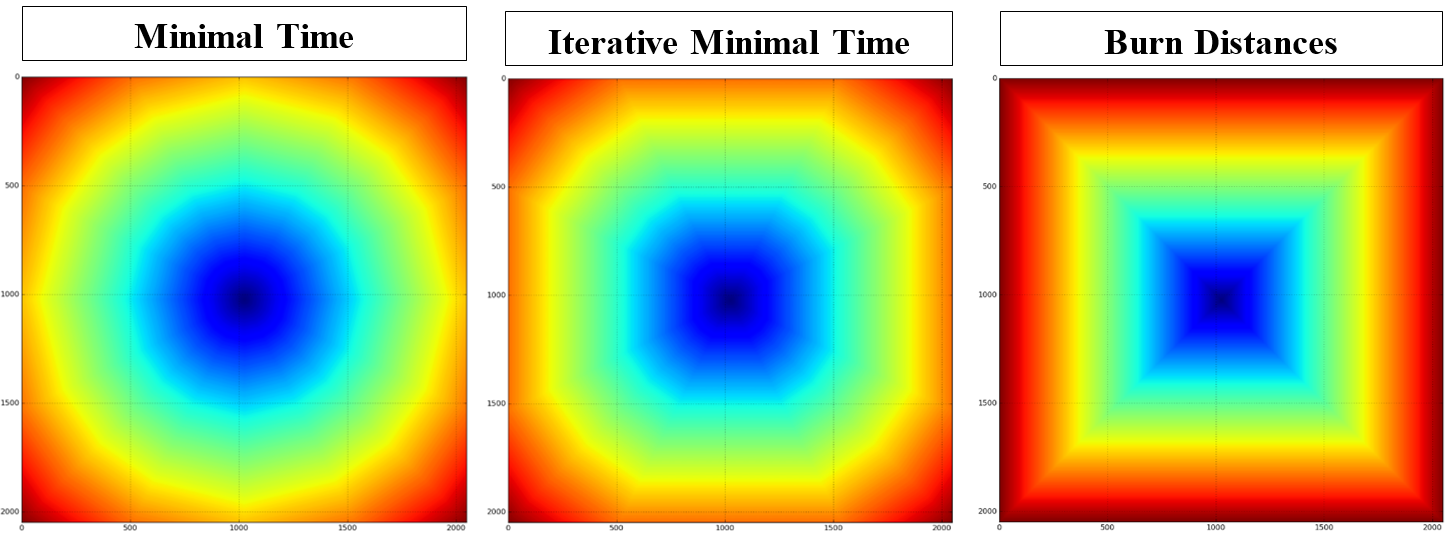
\includegraphics[width=\textwidth,height=4.2cm]{burn_patterns}
  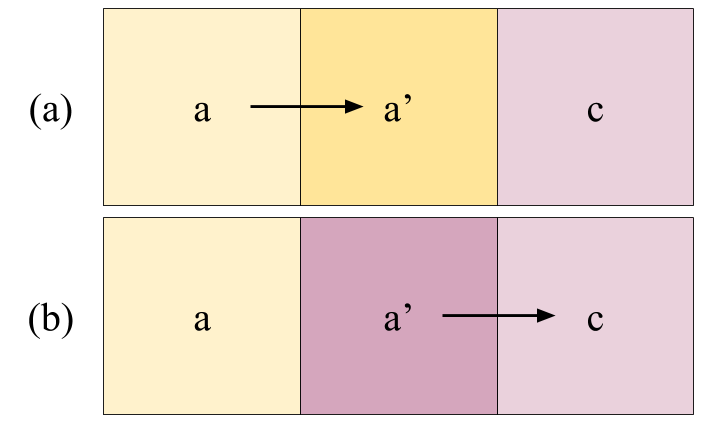
\includegraphics[height=4.2cm]{figures/implementation/read-write-issue.png}
  \caption{An example of the problem syncing thread read access and write access. There is no way to stop one thread writing to another cell before the value is read by another cell.}
  \label{fig:readwrite}
\end{figure}

A secondary kernel was introduced to manage the time update between time steps in the simulation. The secondary kernel was found to be the most efficient solution to this problem. CUDA does not allocate threads in any specific order, which means thread 1 could be the last to finish calculations while thread 1,000 could be the first \cite{cudabyexample}. In order to step through time in the MT propagation method, the timeNext variable needs to be updated after all calculations finish. Since there is no way to ensure which thread would be the last to finish operating on the data, another method for iterating the variable was needed after all threads had finished their computation. The secondary kernel is called after the first terminates, which ensures that all threads have finished their computation before the timeNext variable is updated. Copying the two-element time vector back to the host device and managing the update there was also tested, but it was found to be faster to write a new kernel to update the data without copying anything back to the host device.

\subsection{Iterative Minimal Time}
The IMT kernel is very similar in nature to the MT kernel, but accesses neighbors in the opposite manner. The same data synchronization issues are also found in this kernel, where reading from and writing to the same cells would cause race conditions. A simple example of this problem may be seen in Figure \ref{fig:readwrite}. There is no way to stop a thread from writing to an output position before another thread reads in the data it needs to do its own spread calculations. Figure \ref{fig:readwrite} (a) shows the writing of the value from a to a'. The value that existed before a' was the appropriate value for c to read in to do its calculations. Instead as seen in Figure \ref{fig:readwrite} (b), it is the result value from a that it reads into do its calculations. This error causes race conditions to occur and artifacts to appear in the simulation. Instead of using atomic operations to solve this problem, two time of arrival vectors are passed to the kernel at startup. The two kernels act as an input and output kernel, reading from the former and writing to the latter. This introduces a new problem with maintaining accurate spread data across the input and output vectors. The secondary kernel in the IMT method is both used to copy data from the output back into the input as well as checking for the terminating condition for the simulation. The algorithm for the IMT kernel may be found in Algorithm \ref{alg:IMT}.

\begin{algorithm}[H]
%   \small
  \caption{Iterative Minimal Time Algorithm}
  \label{alg:IMT}
  \begin{algorithmic}
  \FOR{$cell = 0$ to $numCells$}
  \STATE $//$ Check for simulation completion:
  \IF{$|ignTime[cell] - ignTimeNext[cell]| < thresh$}
  \STATE $//$Mark as converged
  \ENDIF
  \IF{$ignTime[cell] > 0$}
  \STATE $ignTimeMin = INF$
  \STATE $//$Propagate Fire
  \FOR{$n = 0$ to $15$}
  \STATE $ROS$ = Compute ROS according to Equation \ref{eq:rate}
  \STATE $ignTimeNew = timeNow + L_n / ROS$
  \STATE $ignTimeMin = MIN(ignTimeNew, ignTimeMin)$
  \ENDFOR
  \ENDIF
  \ENDFOR
  \end{algorithmic}
\end{algorithm}

\section{Fire Acceleration}
A fire does not begin burning at its maximum rate of spread. Instead, it accelerates slowly towards its maximum rate over time as it burns. In this simulator library, fire acceleration is based on the work done by vFire \cite{vFire}. vFire in turn used the model presented by FARSITE \cite{FARSITE}. The formula is a simple logarithmic model that state the rate at some time is dependent on the time allowed for the fire to accelerate to its maximum rate depending on the current conditions of the cell in which it burns. This model was developed by the Canadian Forestry Fire Danger Group and Mcalpine and Wakimoto \cite{accel_canada,accel_mcalpine}. 

Given the maximum spread rate $R_{max}$, the maximum spread rate at time $t$ is given by: 

\begin{equation}
R(t) = R_{max}(1.0 - e^{a_at})
\label{eq:R(t)}
\end{equation}

where $a_a$ is the acceleration constant and is drawn from the fuel model appropriate for the current fire cell. The time $t_{max}$ required to achieve the maximum spread rate given the current spread rate $R$ is given by: 

\begin{equation}
t_{max} = \frac{1.0 - \frac{R}{R_{max}}}{a_a}
\end{equation}

To calculate how much the rate should change per time step, the spread rate for every cell is increased at each time step. The rate of increase $dR$ is given by: 

\begin{equation}
dR = \frac{dt}{t_{max}}(R_{max} - R_{current})
\end{equation}

A newly ignited fire will begin with a spread rate of zero and increase steadily to its maximum rate. Once the maximum spread rate is reached, the simulation does not accelerate past it. As the fire spreads to a new cell, that cell inherits the rate properties of the cell which ignited it. If the maximum spread rate of the newly ignited cell is smaller than the rate it inherits, it is clamped to its maximum. If the rate is slower than the maximum spread rate of the newly ignited cell, it is accelerated using the following equation: 

\begin{equation}
dt = timeOfArrival(thisCell) - max(baseTime, timeOfArrival(ignitingCell))
\end{equation}

The time of arrival issue referred to by Figure \ref{fig:accerr} was a problem caused by acceleration in vFire. However, the time stepping methods in the MT and IMT methods do not have this issue as they have dynamic timestepping, and so they are not bound by the same limitations. The BD method's fix was addressed earlier in the chapter. 

\section{Crown Fire}
The occurrence of crown fires is important for both the overall spread of the fire as well as the phenomena of spotting. Torching occurs when the crown fire spreads from the base of the trees to the top of the trees, and is the moment when the possibility of spotting occurs. The crown fire begins as passive and has the ability to move to an active state, which increases the maximum rate of spread by the fire. The implementation presented in this paper is again based on the implementation found in vFire \cite{vFire}. Their method was based entirely on FARSITE's implementation, which uses Van Wagner's methods found in \cite{wagner1977,wagner1993}. 

In this implemenation, the maximum passive crown rate is given by: 

\begin{equation}
R_{max_{crown}} = 3.34R_{10}
\end{equation}

The necessary components needed for calculating the actual maximum spread rate of an active crown fire in addition to the base propagation are all calculated based on properties found in the fuel model for each cell. The threshold which determines the point at which a passive crown fire is promoted to active (RAC) is given by: 

\begin{equation}
RAC = \frac{3.0}{CBD}
\end{equation}

The reaction intensity ($I_b$) of the fire can be obtained by multiplying the current spread rate by the intensity modifier. The intensity modifier is calculated using the same data which goes into the Rothermel equations.

\begin{equation}
I_b = R * IntensityModifier
\end{equation}

$I_o$ is the threshold intensity for a crown fire to occur. The moment when this threshold is passed is the moment when Torching occurs and a flag must be set for the spotting check. $I_o$ is given as follows: 

\begin{equation}
I_o = (0.010CBH(460 + 25.9M))
\end{equation}

Where CBH is the crown base height and M is the foliar moisture content. The crown base height is stored in one of the input files needed to operate this simulator. In this implementation (as well as the one found in vFire), foliar moisture is simply set to be 1.0. In the context of the simulation, the $I_o$ values only need to be calculated once and are included in the preprocessing phase of the simulator. 

In order to determine the actual spread rate of the fire after crowning, there are two parameters which must be calculated: the crown coefficient ($a_o$), and the surface fuel consumption ($R_o$). $R_o$ can be calculated by using the reaction intensity of the fire, the current rate of spread, and the threshold intensity, given by: 

\begin{equation}
R_o = I_o \frac{R}{I_b}
\end{equation}

The crown coefficient $a_c$ may then be calculated as follows:

\begin{equation}
a_c = \frac{-ln(0.1)}{0.9(RAC - R_o)}
\end{equation}

The crown fraction burned (CFB) of the cell determines the actual maximum current spread rate of the crown fire. The CFB is found using the following equation: 

\begin{equation}
CFB = 1 - e^{-a_c(R-R_o)}
\end{equation}

In order to determine the actual maximum rate of spread, the current rate is added to the $CFB$ that is scaled based on how close to the maximum crown rate the current rate is, as given by: 

\begin{equation}
R_{actual} = R + CFB * (R_{max_{crown}} - R)
\end{equation}

The maximum between this new calculated value and the maximum spread rate for the base fire is the actual value that is passed back as the maximum spread rate of a fire cell containing an active crown fire. 

\section{Spotting}
Spotting is the phenomena that occurs when a fire brand is lofted into the air and blown ahead of the fire to potentially start a new fire ahead of the advancing fire wall. A fire brand is a burning piece of wood from a tree or debris found in the burning fire cell \cite{firereview}. The implementation found in this paper is based on what was developed in the FARSITE fire simulator \cite{FARSITE}. FARSITE uses Albini's 1979 model for spotting propagation to determine the location of the potential new fire \cite{albini}. In this implementation, the fire brands are assumed to be cylinders, which is an approximation to simplify the aerodynamics of the model. Figure \ref{fig:spot_diagram} shows the stages of spotting and will be referenced for the rest of this section as the implementation of spotting is described. 
\begin{figure}%[!b]
\centering
  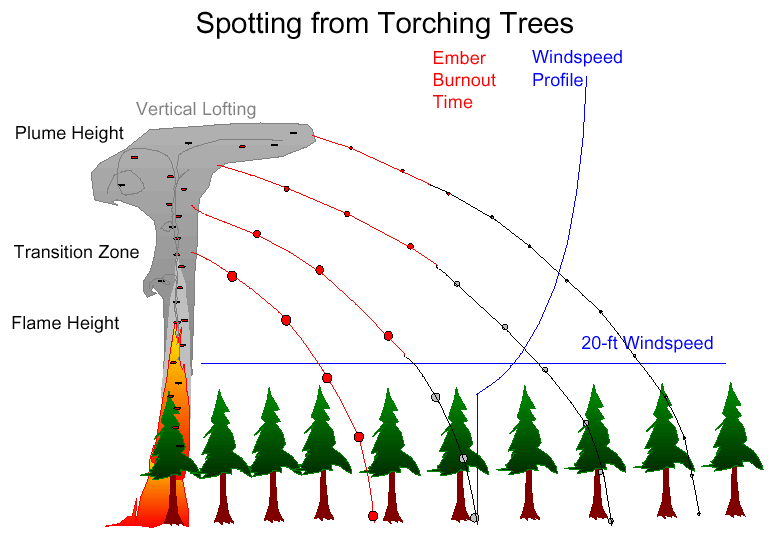
\includegraphics[width=\textwidth]{figures/implementation/spotting_diagram.png}
  \caption{A diagram to represent the phases of spotting, taken from \cite{firebehaveref}.}
  \label{fig:spot_diagram}
\end{figure}

When torching occurs, the spotting calculation can begin. The first important component which needs to be computed is the time it takes for the particle to reach its maximum height $t_t$. $t_t$ is dependent on four time components given by: 
\begin{equation}
t_t = t_0 + t_1 + t_2 + t_3
\end{equation}

Where $t_0$ is the time of steady burning tree crowns. This is a data value that is dependent on the properties of the forest in the cell where spotting is occurring. This value was not available for this work, so a placeholder value was created for the time being and is a constant value for the simulations in the results section of this paper. 

$t_1$ is the time it takes a particle to travel from its point of ignition to the flame tip. This paper makes the assumption that the fire brands originate from the top of the tree crown, but the actual value could be anywhere between the first branches on the tree capable of producing a brand to the tree crown. The equation used to calculate $t_1$ is as follows: 
\begin{equation}
t_1 = 1 - (\frac{z_o}{z_F})^{1/2} + \frac{v_o}{w_F}ln(\frac{1-\frac{v_o}{w_F}}{(\frac{z_o}{z_F})^{1/2} - \frac{v_o}{w_F}})
\end{equation}

Where $z_o$ is the particle height, again assumed to be the crown of the tree. $z_F$ is the flame height. The height of the flame is found as the vertical height from the ground to the tip of the flame \cite{firebehaveref}. $v_o$ is the terminal velocity of the particle and $w_F$ is the flame gas velocity. Again, the data for flame gas velocity was not available to the researchers at this time. A workaround to this problem may be achieved by calculating the ratio of $v_o / w_F$ as:  
\begin{equation}
v_o/w_F = B(D_p/z_F)^{1/2}
\end{equation}

Where $D_p$ is the particle diameter, and $B$ is a constant set to 40. 

The second time section that needs to be calculated $t_2$ is the time it takes the particle to travel between the flame tip and the buoyant plume and is given by: 
\begin{equation}
t_2 = 0.2 + B(\frac{D_p}{z_F})^{1/2}(1 + B(\frac{D_p}{z_F})^{1/2}ln(1 + \frac{1}{1-(\frac{D_p}{z_F})^{1/2}}))
\end{equation}

and $t_3$ is defined as the time it takes the particle to complete its ascent through the buoyant plume. It is given by: 
\begin{equation}
t_3 = \frac{a_x}{0.8\frac{v_o}{w_F}}(ln(\frac{1 - 0.8 \frac{v_o}{w_F}}{1 - 0.8r \frac{v_o}{w_F}}) - 0.8\frac{v_o}{w_F}(r-1) - \frac{1}{2}(0.8\frac{v_o}{w_F})^2(r-1)^2)
\end{equation}

Where: 
\begin{flalign*}
r &= (\frac{(b_x + \frac{z_o}{z_F})}{a_x})^{1/2}\\
a_x &= 5.963\\
b_x &= 4.563
\end{flalign*}

$a_x$ and $b_x$ are constants defined by Albini \cite{albini} and relate to the flame structure. Albini defines the height to which a fire brand will travel as the point in time where the buoyant flow structure of the tree $t_f$ equals $t_t$. The buoyant flow time is defined as: 
\begin{equation}
t_f = t_o + 1.2 + \frac{a_x}{3}((\frac{b_x + \frac{z_o}{z_F}}{a_x})^{3/2} - 1)
\end{equation}
In this implementation, these values had to be approximated in several ways because not all of the necessary data was available. The maximum height was assumed to be constant, and while the equations are implemented and ready for the correct data, it is not yet available. 

A particle will be lofted into the air, and once it reaches its maximum height, the wind then carries it in a direction. If there is no wind in a simulation, the ember would simply fall back to the ground in the cell from which it was launched. Wind is modeled in this library as a 2D vector in each cell of the simulator. The vector contains a magnitude and direction of the wind. The wind vector only contains horizontal data. As in FARSITE's implementation, the fire brand's rate of descent decreases as it falls because as with a real brand, it loses density as it is in the air. Examples of fire brand sizes and their trajectories may be seen in Figure \ref{fig:spot_diagram}. The elevation at any time $t$ is given by: 
\begin{equation}
z(t) = z(0) - v_o(0)(\frac{t}{\tau} - \frac{1}{2}(\frac{t}{\tau})^2)
\end{equation}

Where: 
\begin{flalign*}
\tau &= \frac{4C_dv_o(0)}{K\pi g} \\
K &= 0.0064\\
g &= 9.8 m s^{-2}\\
v_o &= (\frac{\pi g \rho_s D_p}{2C_d\rho_a})^{1/2}\\
\rho_s &= 0.3 g cm^{-3}\\
\rho_a &= 1.2 x 10^{-3} g cm^{-3}\\
C_D &= 1.2
\end{flalign*}

Where $g$ is the gravitational constant, $\rho_s$ is the density of charred wood cylinder, $\rho_a$ is the density of air, and $D_d$ is the drag coefficient of cylindrical particles. 

As the particle descends along its trajectory, its rate of speed in the direction $X$ is determined by the windspeed vector in the cell in which the brand is currently falling. The rate of descent decreases logarithmically as it approaches the top of the tree canopies. 
\begin{equation}
\frac{dX}{dt} = U_H\frac{ln(\frac{z}{z_f})}{ln(\frac{H}{z_f})}
\end{equation}

Where $z$ is the current height of the particle, $H$ is the current height of the forest canopy, and $z_f$ is the friction length of the particle, which is set to $0.4306H$. In this implementation of the paper, there is no modeling of 3-dimensional wind, which means that the wind vector does not change based on height. However, in the interest of presenting a complete model for future work, the windspeed at any height $H$ is given as: 
\begin{equation}
U_H = \frac{U_{20+H}}{ln(\frac{20+1.18H}{0.43H})}
\end{equation}

In this paper, the method for ignition is modeled by a simple probability which is input by the user. However, there are more complex methods for modeling the ignition of a firebrand which impacts the forest floor. Factors such as forest floor fuel type, forest canopy filtering, surface moisture content, and the temperature of the fuel \cite{bradshaw1984,blackmarr1972,bunting1974}. These factors are not examined and are left to future work. Once a fire ignites, it is treated the same as any other ignition source. 

In this paper, spotting introduced new challenges to the development of the library. First, it required new data which was not available to the project. Second, the fire simulations, as seen in the previous sections, propagate the fire by testing to see if a cell has already reached the point of ignition. This point of ignition is determined by the value of the time of arrival for the cell being above zero (which represents the initial fire), and below the value which is set as infinity. In practice this value is the maximum value possibly held by a data type. The problem introduced by spotting is that the time of arrival that is calculated by the spotting kernel is a time of arrival that will occur in the future. As the simulation code was written for the previous sections, the fire would begin to propagate the exact next time tick. To fix this issue, the descent of the falling particle is computed at each time tick with the rest of the simulations and stored in a list of falling embers. The list is updated when one burns out or lands to ignite a new fire, or a new ember needs to be added to the list.  

If the spotting brand's ignition occurs after a cell has already been lit, then it is ignored. If the brand arrives at a time when a cell is not lit, it lights a fire in that cell, which propagates as a normal fire from that point would. 

\section{Simulation Progression}
The simulation has the ability to adapt to the needs of the user. Runtime analysis may be found in Chaper \ref{chapter:results}, which gives an illustration of the impact of adding more features to a simulation. The more features there are to calculate, the longer the runtime will be. However, it is up to the user of the library to decide what is appropriate for their application. The resolution of the fire and desired propagation features allow the user to use the library to create a simulation capable of a flow much like what is seen again in Algorithm \ref{alg:sim2}.

\begin{algorithm}
  \caption{Simulation Progression}
  \label{alg:sim2}
%   \begin{algorithmic}[1] <- this will give you line numb
  \begin{algorithmic}
  \STATE InitializeTerrainData();
  \STATE CalculateSpreadRates();
  \WHILE{Simulation !Complete}
  \STATE RunPropagationSimulation();
  \ENDWHILE  
  \STATE GenerateOutputFile();
  \end{algorithmic}
\end{algorithm}

The specifics of the library's use are left up to the needs of the user. Results for simulation tests may be seen in Chapter \ref{chapter:results}. 
    \chapter{Results}
\label{chapter:results}

\section{Overview}

\section{Running Time Comparison}
\subsection{Overview}
\subsection{Granularity Comparison}
\subsection{Block/Thread Comparison}


\section{Base Spread}

\section{Acceleration}

\section{Crowning}

\section{Spotting}
    \chapter{Conclusions and Future Work}
\label{chapter:conclusions}

\section{Conclusions}


\section{Future Work}
While this work provides a fully-functioning forest fire library, there are several areas where it could be expanded in the future. 

\subsection{Multi-GPU Implementation} 
CUDA provides the ability to program for multiple GPUs at the same time \cite{cuda}. The ability to use multiple GPUs to process the simulation could further improve the runtime. Problems that will arise from implementing the library on multiple GPUs include stitching the simulation together at the edges and triggering memory transfer between GPUs at the point where simulations bleed across the cells being processed on individual GPUs. 

\subsection{Burn Time Selection}
Forest researchers are interested in the carbon footprint caused by a forest fire. This environmental cost is just as important as the physical cost of loss of property and life that can be caused by a wildfire. 

\subsection{Visualization}
In order to better understand the impacts of forest fires in their environment, a visualization is needed. Visualizing the simulation is an important next step for future work of this project. It would allow an interactive environment in which the simulation could exist and be modified dynamically. 
  }


  %\nocite{*}  
  % bibliography
  {
	\newpage
	\baselineskip=13pt
    % \bibliographystyle{IEEEbib} % attempts to order based on appearance
	\bibliographystyle{plain} % attempts to order alphabetically by author
	\addcontentsline{toc}{chapter}{Bibliography}
	\bibliography{bib}
  }
\end{document}
